\begin{figure}[H]
	\centering
	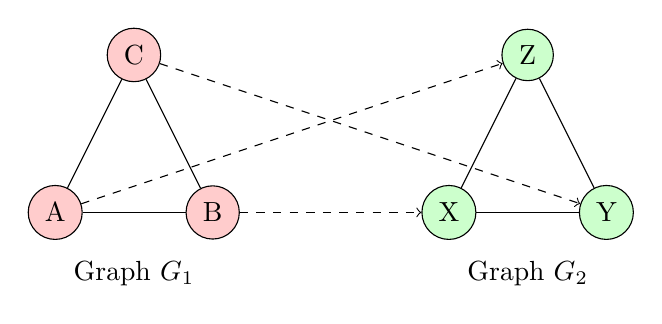
\begin{tikzpicture}
		% Graph Kernels - Left Graph
		\node[circle, draw, fill=red!20] (A) at (0,0) {A};
		\node[circle, draw, fill=red!20] (B) at (2,0) {B};
		\node[circle, draw, fill=red!20] (C) at (1,2) {C};
		\draw (A) -- (B);
		\draw (B) -- (C);
		\draw (C) -- (A);
		\node[align=center, below] at (1, -0.5) {Graph $G_1$};
		
		% Graph Kernels - Right Graph
		\node[circle, draw, fill=green!20] (X) at (5,0) {X};
		\node[circle, draw, fill=green!20] (Y) at (7,0) {Y};
		\node[circle, draw, fill=green!20] (Z) at (6,2) {Z};
		\draw (X) -- (Y);
		\draw (Y) -- (Z);
		\draw (Z) -- (X);
		\node[align=center, below] at (6, -0.5) {Graph $G_2$};
		
		% Dashed lines indicating similarity
		\draw[dashed, ->] (B) -- (X);
		\draw[dashed, ->] (C) -- (Y);
		\draw[dashed, ->] (A) -- (Z);
	\end{tikzpicture}
	\caption{Graph Kernels: Example Graphs with Similar Structures.}
	\label{fig:graph_kernels}
\end{figure}